\subsubsection*{Le matin :}
Réunuion :\\
\begin{itemize}
    \item Environ $n^2$ vecteurs avec $n$ le nombre de dimensions pour l'apprentissage.
    \item Très important que les poids soit positifs (sinon overfiting).
    \item La somme des poids doit valoir $1$.
    \item Les entrées sont comprises entre $0$ et $1$.
\end{itemize}
Pour implementer les conditions precedement citées, la matinée a été passée a coder.
La fonction de perte peut être redéfinie.
Différentes ont été testé, la fonction suivante marche relativement bien :
\begin{equation}
    \label{loss_abs}
    loss(expected, returned) = |expected - returned| + |1 - ||W||\,|
\end{equation}

\subsubsection*{L'après midi :}
Un probleme se pose :\\
Prennons la formule (\ref{choquet}) avec un $n = 2$ (pour simplifier, mais c'est généralisable) :
\begin{align*}
    C_n (X)
    & =
        \sum_{i=1}^{n}
                w_i \times x_i +
            \sum_{i=1}^{n}\sum_{j=i+1}^{n}
            \Big(
                w_{M\,ij} \times \max(x_i,x_j) + w_{m\,ij} \times \min(x_i,x_j)
            \Big)
    &\\
    C_2 (X)
    & =
        w_1.x_1 + w_2.x_2 + w_M.\max(x_1,x_2) + w_m.\min(x_1,x_2)
    &\\
\end{align*}
Etant donné que les données d'apprentissage sont des réels randoms indépendents entre $0$ et $1$ :
\begin{equation}
    \label{proba}
    P(x_1 > x_2) = P(x_1 < x_2) = \frac{1}{2}
\end{equation}
On obtient donc :
\begin{align*}
    C_2 (X)
    & =
        w_1.x_1 + w_2.x_2 + w_M.\max(x_1,x_2) + w_m.\min(x_1,x_2)
    &\\
    <\, C_2 (X) \,>
    & =
        w_1.x_1 + w_2.x_2 + w_M.\frac{x_1 + x_2}{2} + w_m.\frac{x_1 + x_2}{2}
    &
\end{align*}
On obtient donc :
\begin{equation}
    \label{obt}
    <\, C_2 (X) \,> =
        x_1 \times \Big(w_1 + \frac{w_m + w_M}{2}\Big) + x_2 \times \Big(w_2 + \frac{w_m + w_M}{2}\Big)
\end{equation}
Le réseau vas donc essayer d'atteindre les valeurs (\ref{obt}) sans garantir la véracité des coeficients.
Cela est particuilerement visible sur le graphique suivant :
\begin{figure}[H]
    \centering
    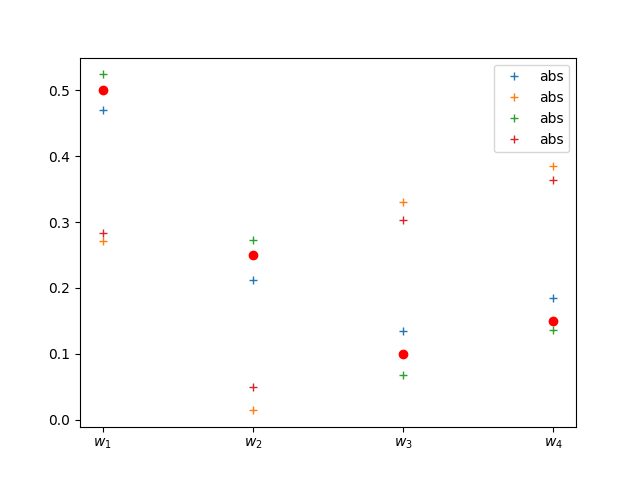
\includegraphics[height=\grand]{sources/data/graphs/pb_adherence.png}
    \label{pb_adherence}
    \caption{Entrainement de 4 réseaux}
    \textit{
        Les points rouge representent les valeurs réelles, les croix representent un entrainement par couleur.
        La fonction d'entrainement est la fonction (\ref{loss_abs})
    }
\end{figure}
Voici le graphique de 4 entrainements indépendents du même réseau de neurones.
Il est bien visible que deux quadruplets de valeurs adherent :
\begin{itemize}
    \item[Les bonne valeurs :] $(0.5, 0.25, 0.1, 0.15)$
    \item[Les valeurs :] $(0.28, 0.2, 0.33, 0.37)$
\end{itemize}
Si on applique la formule (\ref{obt}) on obtient bien :
\begin{table}[H]
    \centering
    \begin{tabular}{|l|l|l|}
        \hline
        Vecteur & $w_1 + \frac{w_m + w_M}{2}$ & $w_2 + \frac{w_m + w_M}{2}$ \\ \hline \hline
        $(0.5, 0.25, 0.1, 0.15)$  & $62.5$ & $37.5$ \\ \hline
        $(0.28, 0.2, 0.33, 0.37)$ &  $63$  &  $37$  \\ \hline
    \end{tabular}
    \label{pb_tab}
    \caption{Valeurs retournées par les réseaux}
\end{table}
On peut voir que les resultats sont sensiblements similaires : le réseau adhère a de mauvaises valeurs.
Pour résoudre ce probleme, il faut ne pas satisfaire (\ref{proba}) et donc tirer un learning set statistiquement différent du testing set.
